\documentclass[main.tex]{subfiles}

\begin{document}
\section{Control System Design Methodology}

The Readout units and the power supply board both require a software end point that essentially controls the entire system. This entails creating a system that can setup and configure the various parts of the system and also monitoring the system and report errors, i.e. we need to create a monitoring and configuration system.

A control system generally is made out of sensors, a controller to control and retrieve data from the sensors, a supervisory computer that manages the process for the sensors, and \gls{hmi} software. The \gls{hmi} software provides access to the data from the sensors to the user and if needed, also allow the user to modify processes in the system.


\subsubsection{SCADA systems}
There are various control systems that have been made over the years in industries such as oil and gas, chemical manufacturing and fabrication. The most common type of control systems in industrial settings is \gls{scada}. \gls{scada} systems have four main functions: data collection, network data communication, data presentation, and remote monitoring and supervisory control\cite{scada_intro}. Although today, many control systems is based on \gls{iot}, which has a similar architecture, but \gls{iot} bases itself on utilizing cloud-networking and processing for its communication infrastructure. Due to lack of wireless communication in the \gls{pct}-project, focus will be on how \gls{scada} systems are developed and what that means for the project.

A \gls{scada} system typically is made out of five components:

\begin{itemize}
    \item Field devices and signals
    \item \acrfull{ppc}
    \item \acrfull{hmi}
    \item Database servers
    \item Communication infrastructure
\end{itemize}

Field devices and signals encompasses all sensors and the actuators that controls them. For \gls{pct}, this includes the \gls{alpide}-chips, temperature and power measurement, and cooling. \gls{ppc} is responsible for automatically controlling the field devices, as well as retrieving data from them and send it to the \gls{hmi}. \gls{hmi} is the software being executed on the main computer and is made of a user interface and database manager. The database server usually contains configuration and monitoring data from the field devices, and the communication infrastructure used in \gls{scada} systems is usually ethernet based.

\subsubsection{Communication network}
There are various communication networks that can be used in a \gls{scada}-system, since all data from the sensors in the \gls{pct} project comes from IPbus, it makes sense for one master computer to receive the data from the IPbus and process it, or send to other computers for processing. (McCrady, 2013) describes in his book of such a communication topology\cite{scada_design}. An example of a \textit{star} topology is shown in \autoref{fig: scada_star}.

\begin{figure}[!ht]
    \centering
    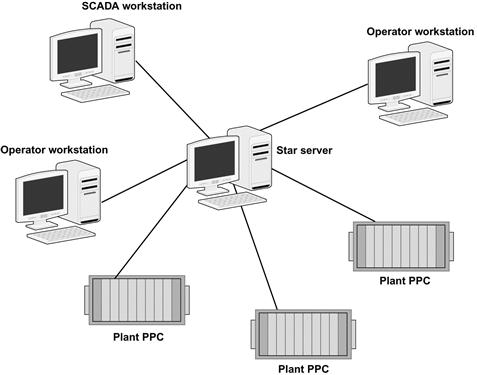
\includegraphics[scale=0.6]{images/scada_topology.png}
    \caption{Example of a star topology communication infrastructure used for SCADA systems\cite{scada_design}}
    \label{fig: scada_star}
\end{figure}
\FloatBarrier

In the \gls{pct}-project, the main computer can be connected to readout, power delivery, and cooling, leading to a \textit{star} topology, even if no other computers are connected.

\subsubsection{I/O Signals}

Important in a \gls{scada} system is to identify all signals to be used and retrieved by the field devices. Knowing all signals to be used in a system will give us an estimate of the requirements of the system as well as aid in the development process.

Power delivery uses a microcontroller to manage power output as well as temperature of the sensors. The microcontroller measures analog voltage(AVDD), digital voltage(DVDD), PWELL voltage, and the temperature of strings. It also have two register for each measurement that dictates the threshold levels, which will make the microcontroller turn off the power if these levels are exceeded. if we include monitoring an error register, and configuring enable signals for the strings, it will then result in 8 input/configuration signals and 8 output/monitoring signals.

\notinmain{Skriv meir om readout og cooling I/O signaler her, ha med ein tabell og kanskje}

\subsubsection{Software documentation}
Another important aspect of such a control system is having a consistent programming standard and complete software documentation. \gls{scada} and similar systems often have a long shelf time, and a well documented system will make maintenance and work in the future be much easier. In general, starting with good software documentation and expanding upon it during the project development will lead to sufficient documentation of the entire system.

A consistent programming standard helps in debugging and in expanding functionality of the system. \gls{oop} is a very common programming paradigm that is used to give structure to programs and increase reusability and maintainability of the code. Systems designed to manage large data acquisition, such as a \gls{pet}-scan system, have in the past used \gls{oop} to design and manage large programs\cite{pet_control_system}, this suggest that this programming structure is viable for the design of the control system in the \gls{pct}-project.

\end{document}

\end{document}